%!TEX encoding = UTF-8 Unicode

\begin{IEEEbiography}[{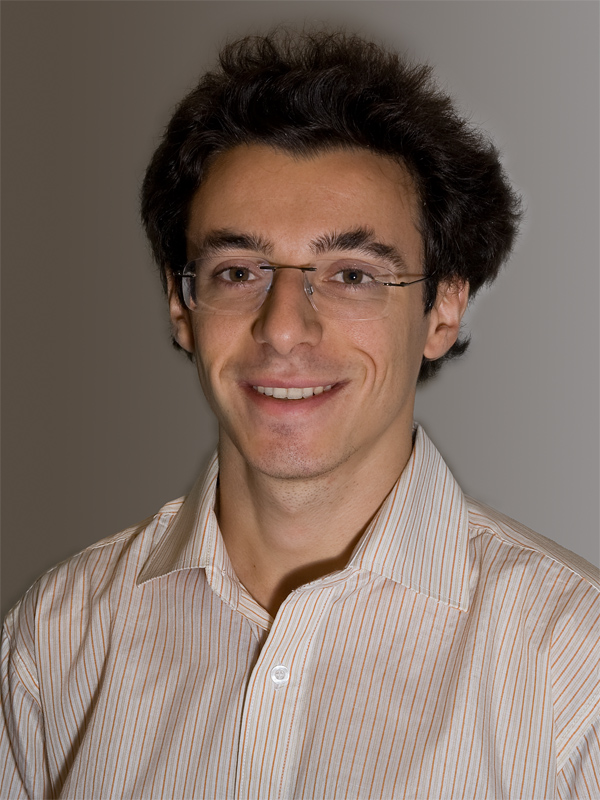
\includegraphics[width=1in,height=1.25in,clip,keepaspectratio]{./author_bios_and_photos/giovanni_saponaro}}]{Giovanni Saponaro}
  (S'11)
  received the B.Sc. degree in computer engineering and the M.Sc. degree~(honors) in computer engineering--artificial intelligence systems from the Sapienza University of Rome, Rome, Italy, in 2005 and 2009, respectively.
  He is currently working toward the Ph.D. degree at the Instituto Superior Técnico, Universidade de Lisboa, Lisbon, Portugal.

  He is a member of the Computer and Robot Vision Laboratory, Institute for Systems and Robotics, Instituto Superior Técnico, Universidade de Lisboa.
  He has participated in the international research project POETICON++, together with linguists, computer vision experts, neuroscientists, and roboticists.
  He has published over ten papers in the diverse areas of cognitive systems, developmental robotics, visual perception of objects and of human body gestures for action recognition.
  His current research interests include visual scene understanding and robot decision algorithms that support \hri{} with highly advanced humanoid robots such as the iCub, and in the presence of uncertainty.
\end{IEEEbiography}

\begin{IEEEbiography}[{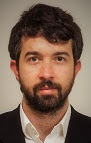
\includegraphics[width=1in,height=1.25in,clip,keepaspectratio]{./author_bios_and_photos/jamone_qmul_100x150px_LD}}]{Lorenzo Jamone}
  (M'13)
  received the M.S. degree (honors) in computer engineering from the University of Genoa, Genoa, Italy, in 2006, and the Ph.D. degree in humanoid technologies from the University of Genoa, Genoa, Italy, and the Italian Institute of Technology, Genoa, in 2010.
  He is a Lecturer of Robotics at the Queen Mary University of London, London, U.K.
  He was an Associate Researcher at the Takanishi Laboratory, Waseda University, Tokyo, Japan, from 2010 to 2012, and the Computer and Robot Vision Laboratory, Instituto Superior Técnico, Universidade de Lisboa, Lisbon, Portugal, from 2012 to 2016.
  He has over~60 publications with an \emph{H}-index of~16.
  His current research interests include cognitive humanoid robots, sensorimotor learning and control, robotic manipulation, and force and tactile sensing.
\end{IEEEbiography}

\begin{IEEEbiography}[{
\includegraphics[width=1in,height=1.25in,clip,keepaspectratio]{./author_bios_and_photos/alexandre_bernardino}}]{Alexandre Bernardino}
  (SM'04)
  received the Ph.D. degree in electrical and computer engineering, in 2004.

  He is an Associate Professor at the Department of Electrical and Computer Engineering and a Senior Researcher at the Computer and Robot Vision Laboratory, Institute for Systems and Robotics, Instituto Superior Técnico, Faculty of Engineering, Universidade de Lisboa, Lisbon, Portugal.
  He has graduated ten Ph.D. students and over 40 M.Sc. students.
  He has participated in several national and international research projects as a principal investigator and a technical manager.
  He has published over~40 research papers in peer-reviewed journals and over~100 papers on peer-reviewed conferences in the fields of robotics, vision, and cognitive systems.
  His current research interests include application of computer vision, machine learning, cognitive science, and control theory to advanced robotics and automation systems.

  Dr. Bernardino is an Associate Editor of the journal \emph{Frontiers in Robotics and AI} and major robotics conferences, such as ICRA and IROS.
  He was a Co-Supervisor of the Ph.D. thesis that won the IBM Prize 2014, and the Supervisor of the Best Robotics Portuguese M.Sc. thesis award of 2012.
  He is currently the Chair of the IEEE Portugal Robotics and Automation Chapter.
\end{IEEEbiography}

\begin{IEEEbiography}[{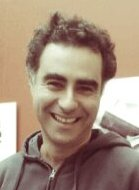
\includegraphics[width=1in,height=1.25in,clip,keepaspectratio]{./author_bios_and_photos/gsalvi}}]{Giampiero Salvi}
  received the M.Sc. degree in electrical engineering from the Sapienza University of Rome, Rome, Italy, and the Ph.D. degree in computer science from the KTH Royal Institute of Technology, Stockholm, Sweden.

  He was a Postdoctoral Fellow at the Institute of Systems and Robotics, Instituto Superior Técnico, Universidade de Lisboa, Lisbon, Portugal.
  He is currently an Associate Professor of Machine Learning and the Director of the Masters Programme in Machine Learning at the KTH Royal Institute of Technology.
  His current research interests include machine learning, speech technology, and cognitive systems.
\end{IEEEbiography}
